\documentclass[aspectratio=169]{beamer}
\usepackage[norsk]{babel}
\usepackage{booktabs}
\usepackage[T1]{fontenc}
\usepackage[utf8]{inputenc}
\usepackage{graphicx,epstopdf,tikz, ifthen}
\usepackage{siunitx, enumerate, xcolor, hyperref}
\usepackage{ enumerate, xcolor}
\usepackage[export]{adjustbox}
\usepackage{circuitikz}
%\usepackage{enumitem}
%\usepackage{enumitem, siunitx}
\usepackage{multicol}
%\usepackage{mathtools}
\usetikzlibrary{decorations.pathreplacing, calc, decorations.pathmorphing, patterns}

\usepackage{minted}

\usetheme[slogan=norsk,style=vertical, mathfont=serif]{NTNU}
\setbeamertemplate{section in toc}[circle]

\title[rl]{Persondata  \\ Tips til mappe}
\date{22. November 2024}
\author{Jonas J. Harang}

%SIunitx
\let\DeclareUSUnit\DeclareSIUnit
\let\US\SI
\let\us\si

\DeclareUSUnit\gallon{gal}
\DeclareUSUnit\inch{in}
\DeclareUSUnit\psi{psi}

\DeclareSIUnit\atm{atm}
\DeclareSIUnit\bar{bar}
\DeclareSIUnit\mmhg{mm Hg}

%%--- tikzcolor for ntnu
\definecolor{NTNUblue}{HTML}{00509e}
\definecolor{NTNUlightblue}{HTML}{6096d0}
\definecolor{NTNUorange}{HTML}{ef8114}
\definecolor{NTNUbrown}{HTML}{cfb887}
\definecolor{NTNUred}{HTML}{b01b81}
\definecolor{NTNUgrey}{HTML}{bebebe}
\definecolor{NTNUcyan}{HTML}{3cbfbe}
\definecolor{NTNUviolet}{HTML}{482776}



%-----------Beamer jonas
%\setbeamertemplate{subsection in toc}[subsections numbered]
\setbeamertemplate{subsection in toc}[subsections unnumbered]
\makeatletter
\newcommand{\SetSectionNumber}[1]{%
\beamer@tocsectionnumber=\numexpr#1-1}
\makeatother

\begin{document}

\begin{frame}
\maketitle
\end{frame}

\begin{frame}{Bruk av personopplysninger}
   \begin{columns}
      \begin{column}{0.6\textwidth}
         \begin{block}{Gode grunner til å trenge persondata}
            \begin{enumerate}[$\bullet$]
               \item {Nødvendig for drift}
               \item {Makedsføring og personalisering}
               \item {Analyse og innsikt}
               \item {Produkt- og tjenesteutvikling}
               \item {Drift og sikkerhet}
               \item {Dokumentasjon og rapportering}
               \item {Kundeservice}
            \end{enumerate}
         \end{block}
      \end{column}
      \begin{column}{0.4\textwidth}
         \begin{figure}
            \begin{centering}
               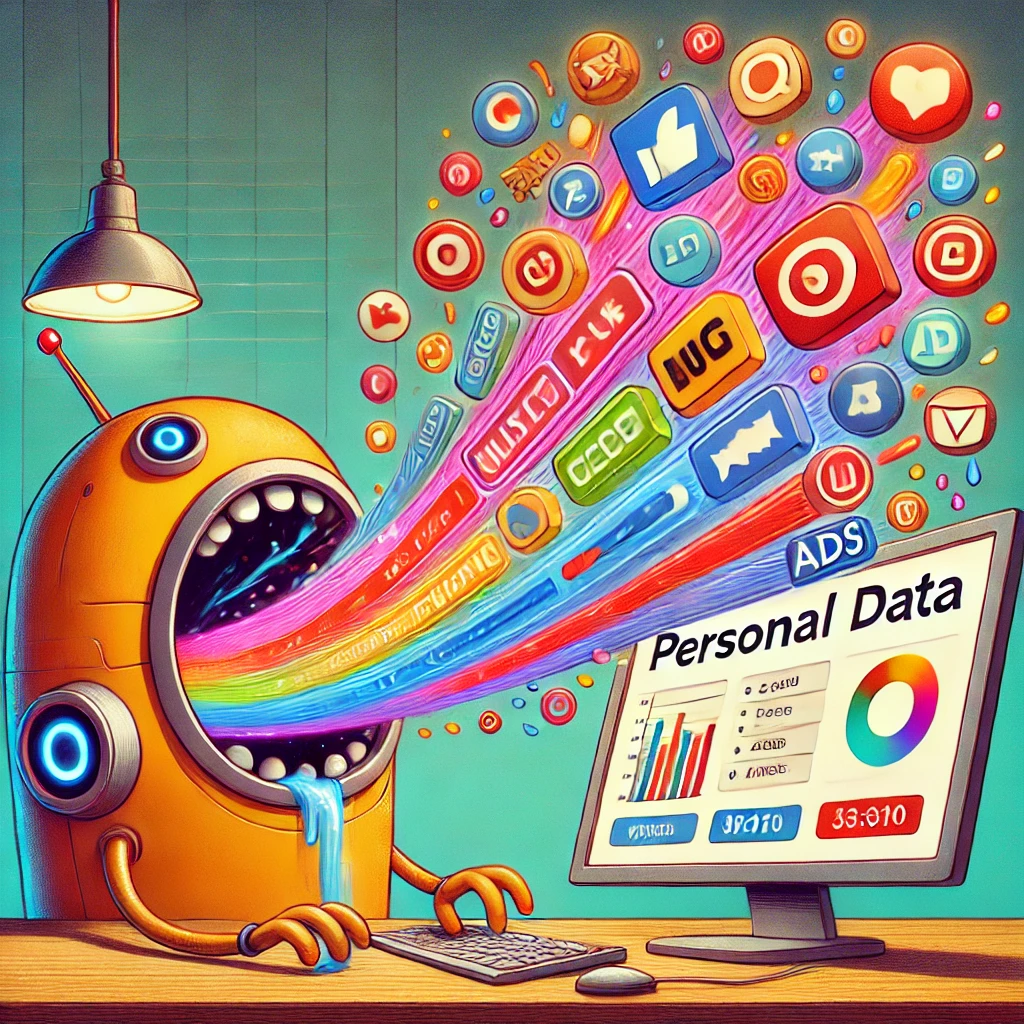
\includegraphics[width=\textwidth]{img/databruk-tall.png}
            \end{centering}
         \end{figure}
      \end{column}
   \end{columns}
\end{frame}

\begin{frame}{Personopplysninger}
   \begin{columns}
      \begin{column}{0.6\textwidth}
         \begin{block}{§Personverforordning artikkel 4}
            \scriptsize
            Personopplysninger er «enhver opplysning om en identifisert eller identifiserbar fysisk person («den registrerte»); en identifiserbar fysisk person er en person som direkte eller indirekte kan identifiseres, særlig ved hjelp av en identifikator, f.eks. et navn, et identifikasjonsnummer, lokaliseringsopplysninger, en nettidentifikator eller ett eller flere elementer som er spesifikke for nevnte fysiske persons fysiske, fysiologiske, genetiske, psykiske, økonomiske, kulturelle eller sosiale identitet»
         \end{block}
      \end{column}
      \begin{column}{0.4\textwidth}
         \begin{figure}
            \begin{centering}
               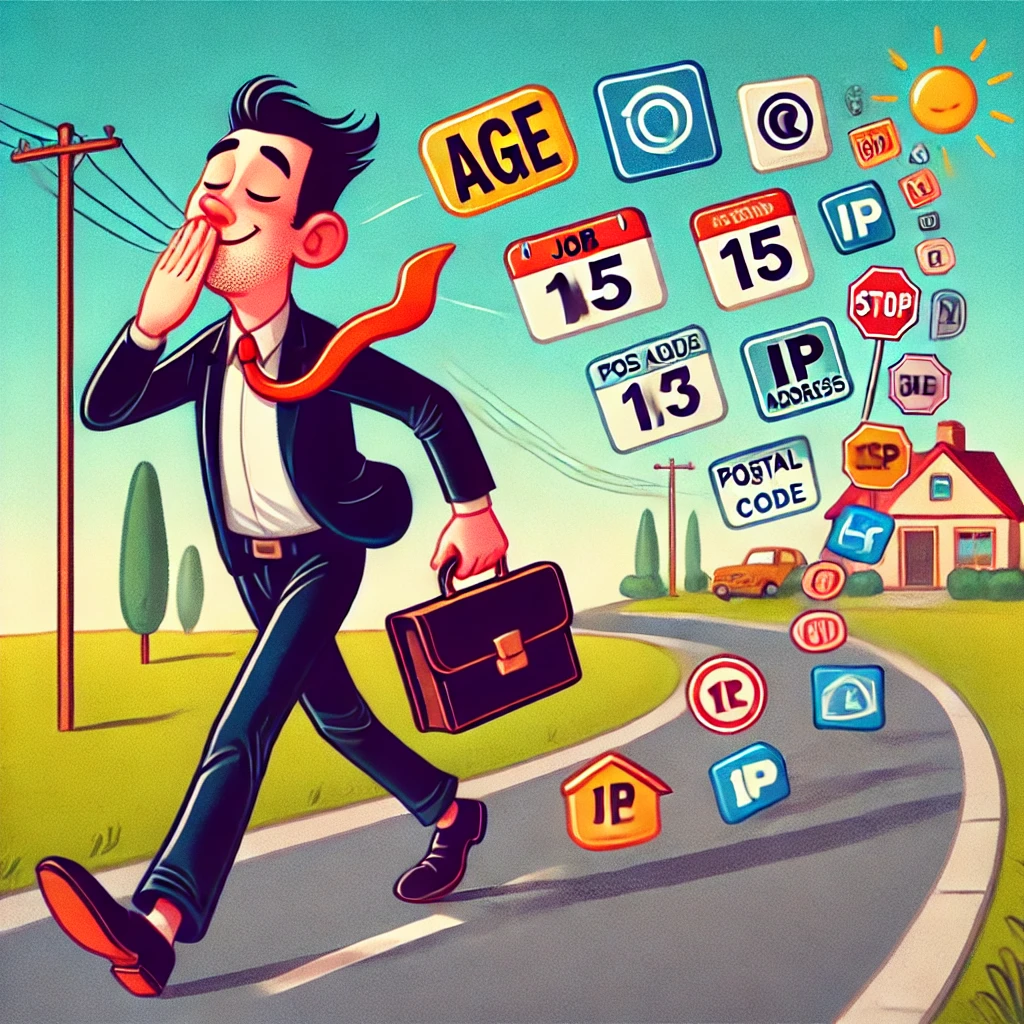
\includegraphics[width=\textwidth]{img/personopplysning.png}
            \end{centering}
         \end{figure}
      \end{column}
   \end{columns}
\end{frame}



\begin{frame}{Begresninger på bruk av personopplysninger}
   \begin{columns}
      \begin{column}{0.6\textwidth}
         Dersom man skal behandle personopplysninger må man ha et \textit{behandlinsgrunnlag} (rettslig grunnlag) 
         \begin{block}{Behandlingsgrunnlag}
            \begin{enumerate}[$\bullet$]
               \item {Rettslig grunnlag til \textit{hver enkelt} personopplysning til hvert enkelt formål}
               \item {Dersom flere kan passe må virksomhet bestemme seg for ett grunnlag}
               \item {Plikt til å informere den enkelte om på hvilket grunnlag personopplysningene behandles}
            \end{enumerate}
         \end{block}
      \end{column}
      \begin{column}{0.4\textwidth}
         \begin{figure}
            \begin{centering}
               
\includegraphics[width=\textwidth]{img/compliance.png}
            \end{centering}
         \end{figure}
      \end{column}
   \end{columns}
\end{frame}

\begin{frame}{Lov om behandling av personopplysninger}
   \begin{block}{Artikkel 6.Behandlingens lovlighet}
Behandlingen er bare lovlig dersom og i den grad minst ett av følgende vilkår er oppfylt:
\scriptsize
      \begin{enumerate}[a.]
         \item	{den registrerte har samtykket til behandling av sine personopplysninger for ett eller flere spesifikke formål,}
         \item {behandlingen er nødvendig for å oppfylle en avtale som den registrerte er part i, eller for å gjennomføre tiltak på den registrertes anmodning før en avtaleinngåelse,}
         \item {behandlingen er nødvendig for å oppfylle en rettslig forpliktelse som påhviler den behandlingsansvarlige,}
         \item {behandlingen er nødvendig for å verne den registrertes eller en annen fysisk persons vitale interesser,}
         \item {behandlingen er nødvendig for å utføre en oppgave i allmennhetens interesse eller utøve offentlig myndighet som den behandlingsansvarlige er pålagt,}
         \item {behandlingen er nødvendig for formål knyttet til de berettigede interessene som forfølges av den behandlingsansvarlige eller en tredjepart, med mindre den registrertes interesser eller grunnleggende rettigheter og friheter går foran og krever vern av personopplysninger, særlig dersom den registrerte er et barn.}
      \end{enumerate}
   \end{block}
Nr. 1 bokstav f) får ikke anvendelse på behandling som utføres av offentlige myndigheter som ledd i utførelsen av deres 
\end{frame}

\begin{frame}{Sensitive personopplysninger}
   Noen personopplysninger skal det mer til å kunne behandle (Særlige kategorier av personopplysninger)
   \begin{enumerate}
      \item {opplysninger om etnisk opprinnelse}
      \item {opplysninger om politisk oppfatning}
      \item {opplysninger om religion}
      \item {opplysninger om filosofisk overbevisning}
      \item {opplysninger om fagforeningsmedlemskap}
      \item {genetiske opplysninger}
      \item {biometriske opplysninger med det formål å entydig identifisere noen}
      \item {helseopplysninger}
      \item {opplysninger om seksuelle forhold}
      \item {opplysninger om seksuell legning}

   \end{enumerate}
   
\end{frame}

\begin{frame}{Hvordan er dette lov?}
   \begin{figure}
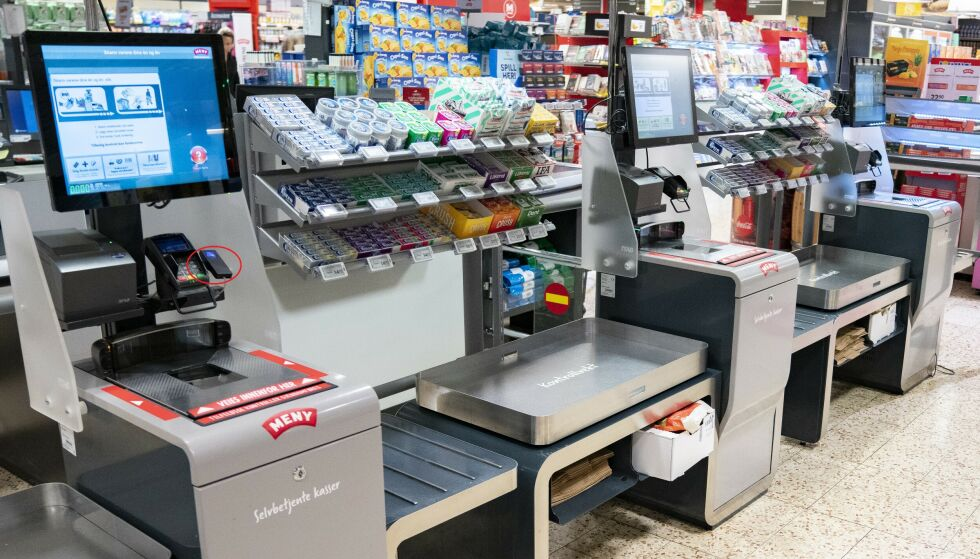
\includegraphics[height=0.7\textheight]{img/fingeravtrykk.jpg} 
   \end{figure}
\end{frame}

\begin{frame}{Anonymisering}
   \begin{itemize}
      \item {Er opplysningene fullstendig anonymisert gjelder ikke det samme \textit{behandlingsansvaret}}
         \begin{itemize}
            \item {Ikke underlagt konsesjonsplikt eller meldeplikt}
            \item {Trenger ikke foreligge rettslig grunnlag, formålsbegresning osv}
         \end{itemize}
      \item {Anonymiseringen må være tilstrekkelig robust og sikkert anonymisert}
   \end{itemize}
\end{frame}

\begin{frame}{Tips og generell tilbakemelding til mappen}
   \begin{block}{Generelt}
      \begin{itemize}
         \item {Gode solide løsninger -- få som ser ut til å ligge under C}
         \item {Jevnt over gode programstrukturer, god variabelbruk, bra visualisering, god bruk av lister og løkker}
         \item {Mangler ofte bruk av i dictionaries, lite vurderingsgrunnlag her -- viktig i dataanalyse sammenheng}
         \item {Mangelfult med kommentarer i koden -- spesielt rundt løkker -- kommenter hva løkken iterer over}
         \item {Generelt tips til forbedring er å gjøre en «personlig vri», (gjerne kun på et av programmene)}
            \begin{itemize}
               \item {Dette for å vise selvstendighet -- at du kan ta i bruk python selvstendig på et "nytt og ukjent" problem}
            \end{itemize}
      \end{itemize}
   \end{block}
\end{frame}

\begin{frame}{KI}
   \begin{itemize}
      \item {Mindre chatGPT-kode enn fryktet :)}
      \item {Husk å redegjøre med kommentarer i koden}
      \item {Eventuelt - om du tar en stor blokk fra chatgpt og gjør masse vesentlige forandringer selv, legg ved "original"-koden til gpt som appendix}
   \end{itemize}
\end{frame}


\begin{frame}{Tips og generell tilbakemelding til mappen}
   \footnotesize
   \begin{columns}
      \begin{column}{0.5\textwidth}
         \begin{block}{Del 1: Populasjonsvekst}
            \begin{itemize}
               \item {For det meste enkelt løst, og det er greit}
               \item {De aller fleste har laget egen funksjon for den logistiske likningen: supert}
               \item {Dersom du ikke har laget et plot av veksten, burde du gjøre det}
               \item {Et tips til rask forbedring er å beregne vekst på mer enn 1 område, og bruke dictionaries som datastruktur til å holde orden på parametre osv}
            \end{itemize}
         \end{block}
      \end{column}
      \begin{column}{0.5\textwidth}
         \begin{block}{Del 1: Sparekalkulator}
            \begin{itemize}
            \item {Mange gode løsninger, jevnt over god programstruktur}
            \item {Mange har fått til grafisk visualisering -- Dersom du ikke har det undersøk om det passer (ikke alltid det gjør det)}
            \item {Tips til forbedring: Ta i bruk flere dictionaries/datastrukturer}
               \begin{itemize}
                  \item {Regn ut saldo for flere personer i en dictionary, og finn rikeste person ved slutt}
                  \item {Samle spareresultat/data for flere scenario i en datastruktur (dictionary) og gjør noe analyse}
               \end{itemize}
            \end{itemize}
         \end{block}
      \end{column}
   \end{columns}
\end{frame}



\begin{frame}{Tips og generell tilbakemelding til mappen}
   \footnotesize
   \begin{columns}
      \begin{column}{0.5\textwidth}
         \begin{block}{Del 1: Databehandling av kunder i sparebank}
            \begin{itemize}
               \item {Typisk godt løst}
               \item {Tips til forbedring: Prøv å gjøre noe som man gjør i pandas "manuelt" med datasettet}
            \end{itemize}
         \end{block}
      \end{column}
      \begin{column}{0.5\textwidth}
         \begin{block}{Del 2: Simulering kundeatferd}
            \begin{itemize}
               \item {Bra og robust på det jevne}
               \item {Tips: Ta med i betraktning dekningsgraden og se også på overskuddet ved salg}
               \item {Tips: Undersøk flere scenarioer og sammenlign (litt på tilbud, veldig på tilbud osv)}
               \item {God mulighet til å vise bruk av dictionaries om det manlger ellers}
               \item {God mulighet til å vise selvstendighet ved å «finne på» noe eget å teste/simulere}
            \end{itemize}
         \end{block}
      \end{column}
   \end{columns}
\end{frame}


\begin{frame}{Tips og generell tilbakemelding til mappen}
   \footnotesize
   \begin{columns}
      \begin{column}{0.5\textwidth}
         \begin{block}{Del 1: Simulering av markedsdynamikk}
            \begin{itemize}
               \item {Typisk godt løst, mye faglig selvstendighet}
               \item {Mulighet til å da i bruk dictionaries også her}
            \end{itemize}
         \end{block}
      \end{column}
      \begin{column}{0.5\textwidth}
         \begin{block}{Del 2}
            \begin{itemize}
               \item {Ser veldig lovende ut}
               \item {Tips: Ikke gjør ting for vanskelig }
               \item {Tips: Prioriter arbeid som gir "spennende" resultat -- grunnlag for diskusjon/analyse}
            \end{itemize}
         \end{block}
      \end{column}
   \end{columns}
\end{frame}


\end{document}

